%!TEX root = ../dokumentation.tex

\chapter{Hardware}

Im folgenden Kapitel werden die elektronischen Hardwarekomponenten, sowie deren Verbindungen untereinander vorgestellt. 

Die einzelnen Komponenten lassen sich in drei große Funktionsbereiche klassifizieren:\\
Der erste Bereich beinhaltet die Distanzbestimmung. Diese wird durch den \ac{LIDAR}-Sensor realisiert.\\
Der zweite Funktionsbereich beschäftigt sich mit dem Ausrichten des Sensors in zwei Achsen. Die Komponenten sind zwei Schrittmotoren und die damit verbundene Ansteuerung durch Motortreiber. \\
Die automatisierte Kalibrierung stellt den dritten Funktionsbereich dar. Dabei wird über eine Lichtschranke die horizontale Ausrichtung des Sensors bei jedem Start der Anwendung auf eine vordefinierte Ausgangsposition gesetzt. Dasselbe wird durch einen Gyrosensor für die vertikale Ausrichtung ermöglicht.

Als Rechen- und Steuereinheit für das gesamte System wird ein Raspberry Pi verwendet. Dieser bietet sich aufgrund des geringen Preises, der vielen \ac{GPIO} Pins und der Unterstützung aller benötigten Datenübertragungsprotokolle an. Zudem reicht die Rechenleistung für das Ansteuern aller Komponenten, sowie für das Auswerten und Speichern der Messdaten aus.\\

\section{Funktionseinheit Distanzbestimmung}

Bei der Auswahl des \ac{LIDAR}-Sensors spielen Preis, Verfügbarkeit, Messfrequenz, Auflösung, Genauigkeit und messbare Entfernung eine Rolle. Im Folgenden werden zwei ausgewählte Sensoren vorgestellt. 


\subsection{TF Mini \ac{LIDAR}}


\begin{wrapfigure}{r}{5cm}
	\vspace{-22pt}
	\hspace{5mm}
	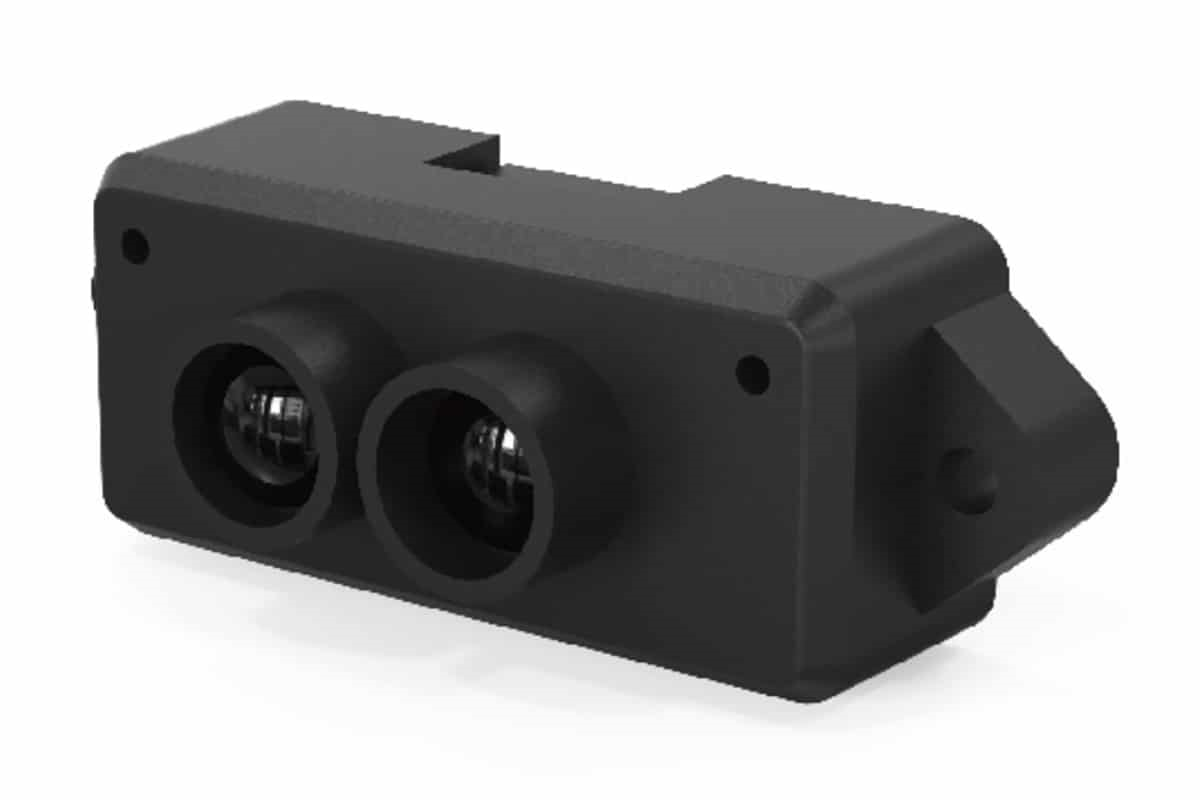
\includegraphics[width=4cm]{images/Hardware/TFmini.png}
	\caption{TF Mini}
	\vspace{-10pt}
	
\end{wrapfigure}

Als Hauptsensor wird ein „TF Mini \ac{LIDAR}“ von dem Hersteller „Seeedstudio“ verwendet. Dieser misst Entfernungen mit auf dem Prinzip der Phasendifferenz wie in Kapitel \ref{sec:phasenverschiebung} beschrieben.\\
Der Arbeitsbereich ist zwischen 30 cm und 1200 cm mit einer Auflösung von 1 cm. Bei Entfernungen kleiner als 600 cm beträgt die Messungenauigkeit 1\%. Zwischen 600 cm und 1200 cm 2\%. Die Messfrequenz beträgt maximale 100 Hz.\\
Der Sensor arbeitet mit einer Versorgungsspannung von 4,5 V – 6 V bei einem durchschnittlichen Stromverbrauch von 120 mA. Das Kommunikation läuft über eine \ac{UART} Schnittstelle mit einer Logikspannung von 3,3 V

Dieser Sensor wurde ausgewählt, da das Preis-Leistung Verhältnis und die Verfügbarkeit sehr gut ist. Zudem reicht der messbare Bereich für den zuvor definierten Standardraum aus. Die Kommunikation über \ac{UART} ist mit dem Raspberry Pi realisierbar. Sensoren mit einer deutlich höheren Messfrequenz sind um ein vielfaches teurer, weshalb aufgrund der Anforderung eines kostengünstigen Systems die Messfrequenz von 100 Hz  ausreichend sein muss. Zusätzlich wird dadurch nicht die Qualität des Ergebnisses beeinflusst. Die niedrigere Messfrequenz beeinträchtigt nur die Geschwindigkeit, mit der ein Raum vermessen werden kann. \\
Der Sensor ist 42 x 15 x 16 mm groß, wodurch er sehr gut auf der dafür vorgesehenen Aluminiumhalterung montiert werden kann. \cite{TFMINI}


\subsection{VL53L1X} \label{sec:VL53L1X}

Als alternativer, kostengünstigerer Sensor wird der \ac{ToF}-Sensor VL53L1X verwendet. Der Sensor nutzt das Prinzip der Lichtlaufzeitmessung. Es können Distanzen von bis zu 400 cm mit einer maximalen Frequenz von 50 Hz gemessen werden. Die Kommunikation erfolgt über \ac{I$^{2}$C}. \\
Die Versorgungsspannung beträgt zwischen 2,6 und 3,5 V. Sowohl der Erfassungswinkel als auch der interessante Entfernungsbereich kann softwaretechnisch eingestellt werden. \cite{VL53L1X}

Der Arbeitsbereich ist von dem eingestellten Distanzmodus abhängig. Man kann wie in Tabelle \ref{distanzmodi} dargestellt zwischen drei Modi auswählen. Die Tabelle zeigt zudem die maximal messbare Distanz für den jeweiligen Modus in Abhängigkeit von dem Umgebungslicht. Der Modus für kurze Distanzen ist  Umgebungslicht unempfindlich. Bei den Modi für mittlere bis hohe Distanzen reagiert der Sensor sehr stark auf Umgebungslicht. Die maximal zu messende Distanz beträgt bei hohem Umgebungslicht nur noch ca. 75 cm. 

\begin{center}
	\begin{tabular} [H] {|c|c|c|}
		\hline
		\textbf{Distanz Modus} & \textbf{max. Distanz (abgedunkelt)}	& \textbf{max. Distanz (Umgebungslicht)} 	 \\ \hline
		Kurz	&  136 cm		& 135 cm\\ \hline
		Mittel  &  290 cm	  	& 76 cm	\\ \hline
		Lang 	&  360 cm		& 73 cm	\\ \hline
				
		\end {tabular}
		\captionof{table}{Distanzmodi VL53L1X}
		\label{distanzmodi}
	\end{center}

In der späteren Anwendung wird der Modus für große Distanzen benötigt. Daher sollten während der Messung potentielle Fehlerquellen durch Umgebungslicht vermieden werden.

Die Genauigkeit der Messung hängt wie in Abbildung \ref{VL53L1X} zu sehen von der Messfrequenz ab. Die Abbildung zeigt das Verhalten bei unterschiedlichen Frequenzen. Dabei wird auf die Genauigkeit des Sensors, die maximal messbare Entfernung und die Replizierbarkeit der Messwerte eingegangen. ''Timing Budget'' ist dabei die Zeit, die benötigt wird, um einen Messwert aufzunehmen. Die Frequenz lässt sich daraus mit dem Kehrbruch berechnen.
STDEV steht für "standard deviation" oder auch Standardabweichung. Dieser Wert gibt die Streubreite der gemessenen Werten um den tatsächlichen Wert an. Je höher dieser Wert, desto geringer ist die Genauigkeit des Sensors. \\ 
 
Das obere Diagramm zeigt das Verhalten des Sensors bei einer Messfrequenz von 30,3 Hz. Bei dieser Frequenz kann unter perfekten äußeren Bedingungen nur eine maximale Distanz von 310 cm erreicht werden. Zudem ist die Genauigkeit des Sensors am schlechtesten. Mit kleiner werdender Messfrequenz nimmt die Genauigkeit zu und der maximal Messbare Distanz beträgt bei entsprechenden Messverhältnissen 400 cm. Gute Messverhältnisse sind möglichst wenig Umgebungslicht und gut reflektierende Gegenstände. \cite{VL53L1X_manual}

\begin{figure}[H]
	\centering
	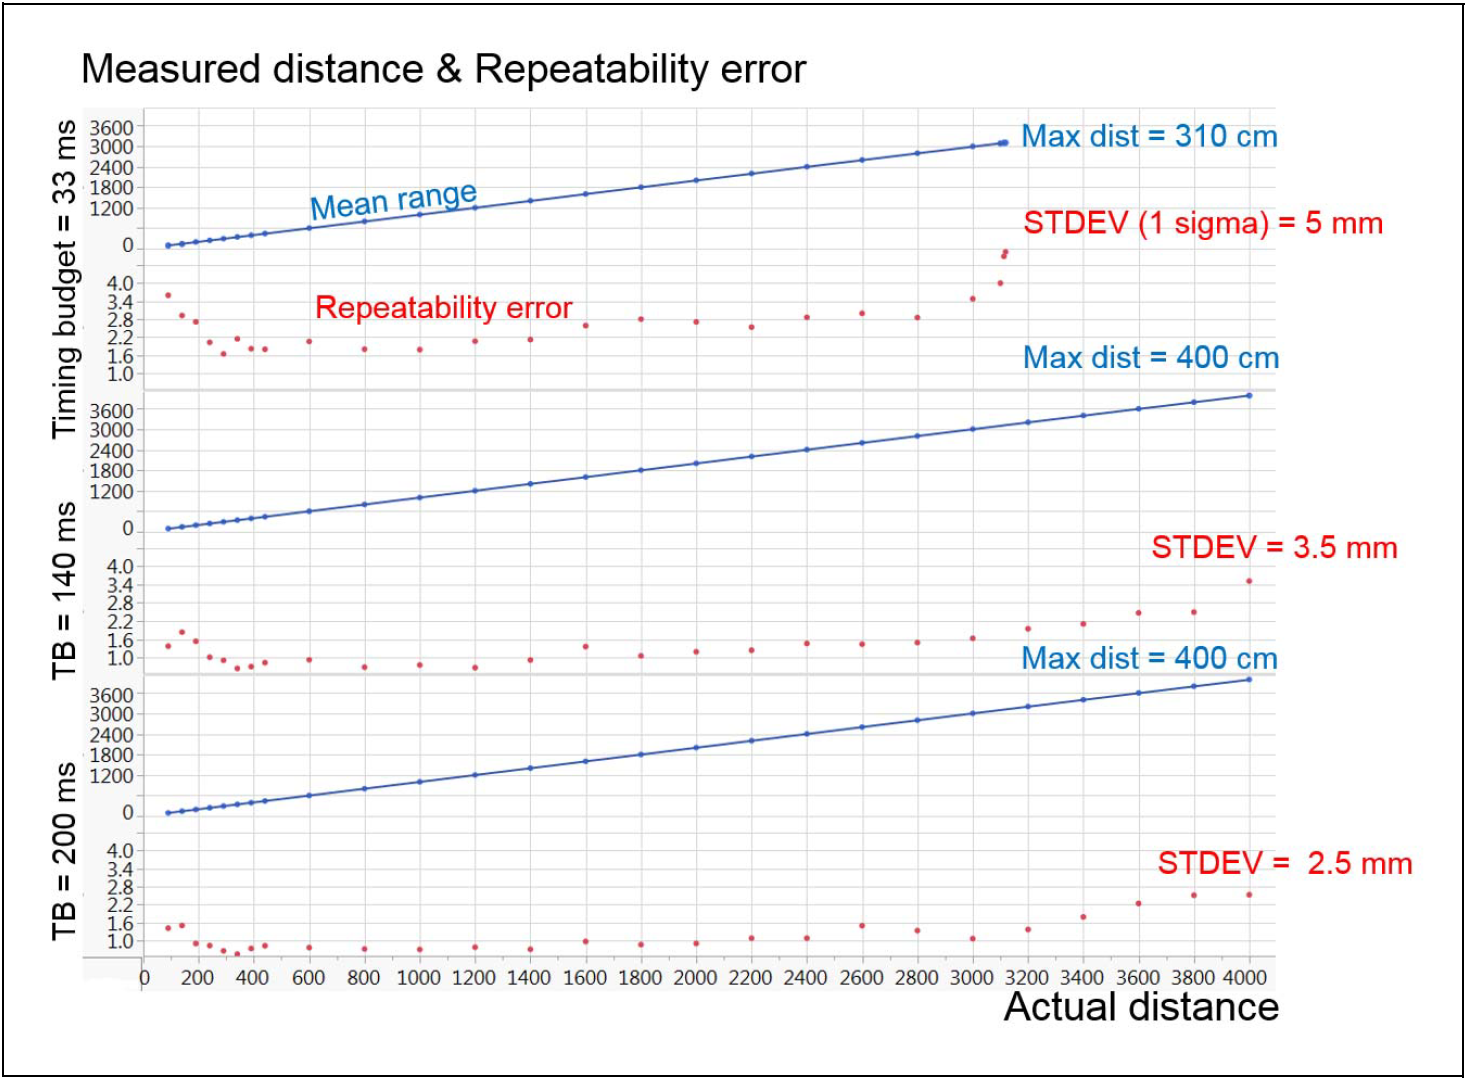
\includegraphics[width=0.75\textwidth]{images/Hardware/VL53L1X_Messfrequenz}
	\caption{Abhängigkeit der Genauigkeit des VL53L1X Sensors von der Messfrequenz}
	\label{VL53L1X}
\end{figure}


Der Sensor ist mit 4,9 x 2.5 x 1.56 mm sehr klein. Zudem müssen 12 Pins auf der Unterseite verlötet werden. Mangelnder Ausrüstung zum Löten solchen Chips, wird ein bereits verbauter Sensor auf einer Platine verwendet. Auf der Platine sind zudem benötigte Widerstände und Kondensatoren verbaut. Werden die 12 herausgeführten Pins der Platine verwendet, ist der Sensor um 90 Grad vertikal verdreht und kann nicht auf der dafür vorgesehenen Adapterplatte der Mechanik montiert werden. Deshalb wird eine weiter Adapterplatine entworfen, auf welche die Platine mit dem Sensor aufgesteckt werden kann und somit um 90 Grad gedreht wird.



-- BILD, Schaltplan, Board...


Fazit: Sensor nicht so gut, aufpassen bei Messen wegen äußeren Bedingungen



\subsection{Tabellarischer Vergleich der Sensoren}

Eine tabellarischer Auflistung der relevanten Daten der beiden ausgewählten Sensoren vereinfacht den direkten Vergleich für spätere Auswertungen. Neben vor allem technischen Daten wird auch der Preis in Tabelle \ref{vergleich} aufgenommen.

\begin{center}
	\begin{tabular} [H] {|c|c|c|}
		\hline
		\textbf{} 				& \textbf{Tf Mini LIDAR}	& \textbf{VL53L1X} 	 \\ \hline
		Preis [€]				&  35-40					& 10			\\ \hline
		Arbeitsbereich [cm]		&  30 - 1200   				& 3-400			\\ \hline
		max. Messfrequenz [Hz]	&  100						& 50 			\\ \hline
		Messungenauigkeit [\%]	&  1-2 						& <1			\\ \hline
		Schnittstelle 			&  \ac{UART}				& \ac{I$^{2}$C}\\ \hline
		Versorgungsspannung [V] &  4,5 - 6 					& 2,6 - 3,5		\\ \hline
		
		\end {tabular}
		\captionof{table}{Tabellarischer Vergleich TF Mini und VL53L1X}
		\label{vergleich}
	\end{center}

Es gilt zu beachten, dass sich beim Sensor VL53L1X einige Werte gegenseitig ausschließen. So ist bei der Messfrequenz von 50 Hz beispielsweise keine Entfernung von 400 cm messbar. Diese gegenseitigen Einschränkungen sind in Kapitel \ref{sec:VL53L1X} aufgeführt und erklärt.

 

\section{Funktionseinheit Ausrichtung des Sensors}

Der Sensor wird durch je einen Schrittmotor in der horizontalen als auch vertikalen Richtung bewegt. Die vertikale Ausrichtung erfolgt dabei direkt. Der Sensor ist über eine Adapterplatte mit der Welle des Schrittmotors verbunden. Dadurch werden Bewegungen des Schrittmotors 1:1 auf den Sensor übertragen.\\
Die horizontale Ausrichtung erfolgt zusätzlich über ein Getriebe mit einem Riemen zur Kraftübertragung. Das Übersetzungsverhältnis entspricht 1:6. 

\subsection{Schrittmotoren}
Das drehen der Basis übernimmt ein bipolarer Hybrid-Schrittmotor der Bauform Nema 17 und einem Vollschrittwinkel von 1.8°. Der Maximalstrom beträgt 1.2 A pro Phase bei einer Spannung von 4V.\\
Dieser Motor wurde gewählt, da er genug Drehmoment aufbringt, um die gesamte Basis drehen zu können. Das hohe Haltemoment verhindert ungewolltes Verdrehen der Basis während der Messung. Dadurch ist das System fehlerresistenter auf äußere Einflüsse. 


Zum Kippen des Lidar-Sensors wird ebenfalls ein bipolarer Hybrid-Schrittmotor verwendet. Dieser Motor befindet sich auf der sich drehenden Basis. Der Schwerpunkt des Motors befindet sich dabei unumgänglich einige Zentimeter neben der Drehachse. Deswegen sollte der Motor möglichst wenig Gewicht aufweisen, um die Unwucht so klein wie möglich zu halten.
Zum vertikalen Kippen des Sensor wird nicht so viel Kraft benötigt, als für das Drehen der gesamten Basis. Auf Grund dessen reicht die Bauform Nema 11. Diese Bauform ist deutlich kleiner und dadurch leichter.
Das Haltemoment reicht aus, um ungewolltes vertikales Verdrehen zu vermeiden.


\subsection{Schrittmotortreiber}
Zur Ansteuerung der Schrittmotoren wird der Schrittmotortreiber A4988 verwendet. Dieser ist bereits auf einer Trägerplatine mit Teilen der äußeren Beschaltung verbaut.\\
Der Motortreiber ermöglicht es, bipolar Schrittmotoren mit eine Motorspannung von 8 V bis zu 35 V und einem maximalen Phasenstrom von 2 A anzusteuern.
Zudem sind mit dem Motortreiber Mikroschritte realisierbar. Dabei sind halb, viertel, achtel und sechzehntel Schritte möglich. Der maximale Ausgangsstrom ist über einen Potentiometer auf der Trägerplatine stufenlos einstellbar. 

--ToDO: Zeichnung --



Der Motor wird Spulenweise an den Motortreiber angeschlossen. Dabei wird Pin 1A und 1B sowie 2A und 2B über jeweils eine Spule des Schrittmotors verbunden.
Die Versorgungsspannung wird über ein 12 V Tischnetzteil bereitgestellt. Diese wird zusätzlich mit einem Stützkondensatoren geglättet, um Spannungsspitzen auszugleichen.
Als Kontrolleinheit für den Motortreiber dient ein Rapsberry Pi. Die Logikspannungsversorgung des Treibers wird mit einem 5 V Ausgang des Raspberry Pi’s verbunden.
Step, Dir, sowie MS1-MS3 werden mit GPIO’s verbunden. Der Logikpegel an dem DIR-Pin legt die Bewegungsrichtung des Motors fest. Ein toggelndes Signal am Step Pin führt zur Rotation des Motors. Pro Steigende Flanke dreht sich der Motor um an den MS1-MS3 eingestellte Schrittweite weiter. 
MS1-MS3 dienen zum Einstellen der Schrittweite. Die Kombination der Logiklevel entscheidet dabei über die Schrittweite. Theoretisch wären somit 2hoch3 also 8 Komoinationen möglich. Da jedoch nur fünf Einstellunen benötigt werden, sieht die Wahrheitstabelle Folgendermaßen aus:

Tabelle:

\begin{center}
	\begin{tabular} [H] {|c|c|c|c|}
		\hline
		\textbf{MS1} & \textbf{MS2}	& \textbf{MS3} 		& \textbf{Auflösung} \\ \hline
		Low & Low	& Low		& Vollschritt\\ \hline
		High & Low 	& Low  		& Halbschritt	\\ \hline
		Low & High  & Low 		& viertel Schritt 	\\ \hline
		High & High	& Low 		& achtel Schritt 	\\ \hline
		High & High	 &  High	& sechzehntel Schritt	\\\hline
	
		\end {tabular}
		\captionof{table}{Schrittweite}
		\label{Mikrostepping}
	\end{center}



Um Beschädigungen an den Schrittmotoren zu vermeide, muss der maximale Strom durch die Spulen begrenzt werden. Dies kann man über einen Potentiometer auf der Oberseite des Treiberbausteines machen. Dafür wird die Referenzspannung zwischen dem Potentiometer und Masse gemessen. Mit der Formel : Current Limit = VRef *2 kann der maximale Strom ausgerechnet werden.
Unterschiedliche Bauweisen des Treiberbausteines führen aber oftmals dazu, dass die Formel nur als grober Richtwert gewertet werden kann. Nach der groben Einstellung des Stromlimits sollte man den Strom bei aktivem Motor messen und gegebenfalls noch anpassen.
Ändert man die Schrittweiten, ändert sich das Limit etwas…

Pro Motor wird ein Motortreiber auf der Platine verwendet.



\section{Funktionseinheit Kalibrierung}

\subsection{Lichtschranke}
Zum automatischen Positionieren der Basis wird eine Infrarot Lichtschranke verwendet. Diese befindet sich direkt unter dem Ritzel und detektiert das Durchlaufen des daran befestigten Kalibrierzapfens.
Auf dem Lichtschrankenmodul ist LM393..
Das Modul benötigt eine Versorgungsspannung von 5V. Zudem wird der Ausgangspin mit einem GPIO Pin des Raspberry Pis verbunden. An diesem Ausgang liegt ein digitales Signal an, welches den Status der Lichtschranke darstellt. Liegt ein HIGH- Signal an, befindet sich etwas in der Lichtschranke und sie ist unterbrochen. Wechselt dieser Wert auf einen LOW Pegel, so ist die Lichtschranke nichtmehr unterbrochen.

\subsection{Gyroensor}






\section{Platinen}



\section{Abwärtswandler}

Da für einige Komponenten eine Spannung von 5V benötigt wird, muss die Versorgungsspannung von 12 V verkleinert werden. Dazu wird ein Abwärtswandler verwendet. Über ein Potentiometer auf der oberseite des Moduls kann die Ausgangsspannung eingestellt werden. (MINI-360)






